\subsubsection{Deconvolution}
This tool does more than simply reducing the effect of energy resolution but will still be referred to as a deconvolution operation. Deconvolution in this sense is more similar to reconstruction as in image reconstruction in nuclear medicine, it employs the ML-EM algorithm. By using a detector response matrix, most simply acquired using Monte Carlo-simulations, the effects of the detector resolution, scattering in the detector and other effects can be reduced. The response matrix represents the expected detector response to a photon emitted at a certain energy, see \autoref{tab:response_matrix_schema} and section \ref{sec:}

\begin{figure}[H]
    \centering
    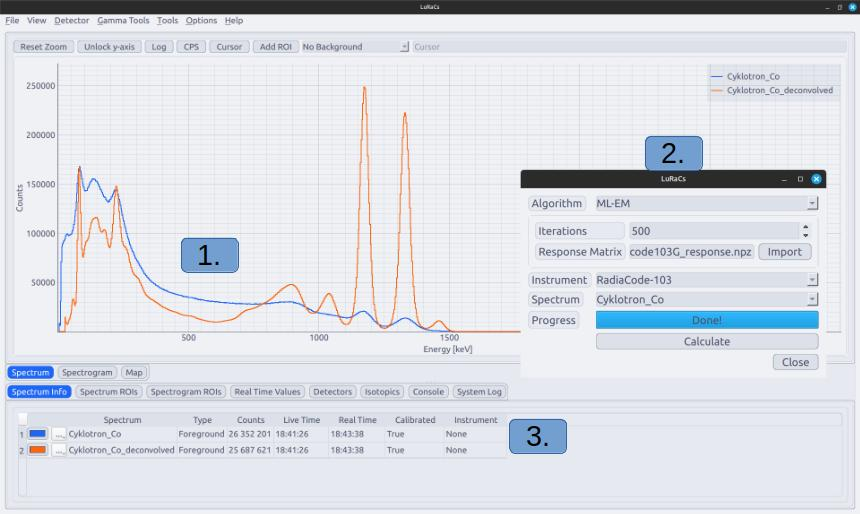
\includegraphics[width = .9\linewidth]{images/interface/gtools_deconvolution.jpg}
    \caption{A Co-60 spectrum deconvolved using ML-EM and a response matrix for a Radiacode-103G detecting a parallel beam of monoenergetic photons.}
    \label{fig:gtools_deconvolution}
    \begin{flushleft}
        \begin{enumerate}
            \item The original Co-60 spectrum  in blue and the deconvolved spectrum in orange.
            \item Control window for the deconvolution operation, see \autoref{tab:gtools_deconvolution}.
            \item The deconvolved spectrum is added as new spectrum, copying information from the original.
        \end{enumerate}
    \end{flushleft}
\end{figure}

\begin{table}[H]
    \centering
    \caption{Description of the deconvolution window.}
    \label{tab:gtools_deconvolution}
    \begin{tabular}{p{.3\textwidth}p{.64\textwidth}}
    \toprule
    \textbf{Field} & \textbf{Description} \\ \midrule
        Algorithm & Which algorithm should be used. Options are \texttt{ML-EM} (use this) and \texttt{Generalized Richardson-Lucy}. \\
        Iterations & The number of iterations the algorithm should run. \\
        (ML-EM) Response Matrix & The path to a .npz file containing the detector response matrix to be used. \\
        Instrument & Instrument providing information for the algorithm. For instance, \texttt{Generalized Richardson-Lucy} is based on the resolution saved in the instrument. \\
        Spectrum & Which spectrum should the operation be executed on. \\
        \bottomrule
    \end{tabular}
\end{table}